\chapter{Extended Language Models}

This chapter describes several recently proposed NLM architectures designed to tackle the rare word prediction problem and highlights the main similarities and differences among them. We also introduce our proposed model called ``Sentinel Mixture''.

\section{Attention Models}
\label{sec:attention}

Although the concept of attention that we are going to introduce is not directly concerned with rare word prediction, it will help us lay the foundations for the subsequent models as they take inspiration from it.

\subsection{Original Formulation}

Attention models were firstly developed in the field of neural machine translation (NMT) in the seminal paper \cite{bahdanau2014neural}. At that time, most of the proposed NMT models belonged to a family known as ``encoder-decoders'' \cite{sutskever2014sequence}. These models consist of two parts: first an encoder (a deep bidirectional LSTM network) compresses the source sentence (specifically the embeddings for each word) $\{\mathbf{i}(1), \mathbf{i}(2), \cdots, \mathbf{i}(n_i)\}$ into fixed-length vector representation $\mathbf{c}$. This is done by sequentially processing the sentence with a recurrent network and taking the last hidden state $\mathbf{h}(n_i)$ as $\mathbf{c}$ (\autoref{eq:encoder}).

\begin{equation} \label{eq:encoder}
	\begin{gathered}
		\mathbf{h}(t) = \text{LSTM}(\mathbf{i}(t), \mathbf{h}(t-1)) \\
		\mathbf{c} = \mathbf{h}(n_i)
	\end{gathered}
\end{equation}

Then a decoder (also a deep LSTM network) outputs a translation sentence $o=\{o(1), o(2), \cdots, o(n_o)\}$ using $\mathbf{c}$ as its first input. As shown in \autoref{eq:decoder}, in a similar way as the RNLM models that we saw in \autoref{sec:rnn}, the probability of outputting a word at step $t$ is obtained as the vocabulary softmax of an affine transformation of the hidden state $\mathbf{s}(t)$.

\begin{equation} \label{eq:decoder}
	\begin{gathered}
		\mathbf{s}(t) = \text{LSTM}(\mathbf{o}(t-1), \mathbf{s}(t-1)) \\
		p(o) = \prod_{t=1}^{n_o} p(o(t)|\{o(1), \cdots, o(t-1)\}, \mathbf{c}) \\
		p(o(t)|\{\mathbf{o}(1), \cdots, \mathbf{o}(t-1)\}, \mathbf{c}) = \text{softmax}(W_o \mathbf{s}(t) +\textbf{b}_o)
	\end{gathered}
\end{equation}

A potential problem for this architecture is the fact that all the necessary information from a source sentence has to be encoded into the vector $\mathbf{c}$. Hence, this may make it difficult for the model to deal with long sentences. Instead the decoder is allowed to access the full sequence of the encoder's hidden states $\{\mathbf{h}(1), \mathbf{h}(2), \cdots, \mathbf{h}(n_i)\}$, as shown in \autoref{fig:nmtAttention}.

\begin{figure}[H]
	\centering
	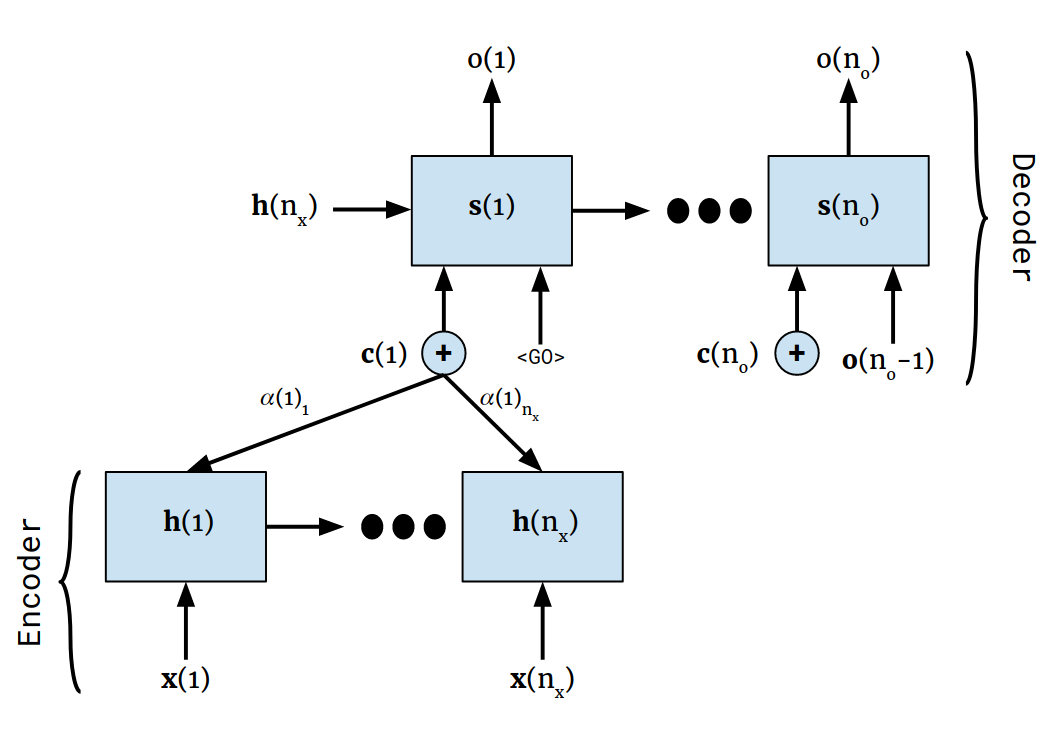
\includegraphics[scale=0.28]{nmt}
	\captionof{figure}{Attention NMT model}
	\label{fig:nmtAttention}
\end{figure}

In this new architecture the decoder is provided with an additional input, the context vector $\mathbf{c}(t)$. For each step $t$ of the decoder, it is calculated in the following way:

\begin{equation} \label{eq:nmtAttention}
	\begin{gathered}
		\mathbf{e}(t)_k = e_{tk} = \mathbf{v_a}^{\top} \tanh(W_a \mathbf{s}(t-1)+U_a\mathbf{h}(k)), \; \forall k \in 1, \cdots , n_i  \\
		\boldsymbol{\alpha}(t)_k = \alpha_{tk} = \frac{e^{e_{tk}}}{\sum_{j}e^{e_{tj}}}, \; \forall k \in 1, \cdots , n_i  \\
		\mathbf{c}(t) = \sum_{k=1}^{n_i} \alpha_{tk} \mathbf{h}(k)
	\end{gathered}
\end{equation}

where $\mathbf{e}(t),\boldsymbol{\alpha}(t) \in \mathbb{R}^{n_i}$, $W_a \in \mathbb{R}^{h \times h}$, $U_a \in \mathbb{R}^{h \times 2h}$, $\mathbf{h}(t) \in \mathbb{R}^{2h}$ and $\mathbf{v_a},\mathbf{s}(t),\mathbf{c}(t) \in \mathbb{R}^{h}$. 

First, a vector of attention scores $\mathbf{e}(t)$ is calculated in order to see how much each source word should be ``attended'' with respect to the current decoder step. These are obtained with a single-layer multilayer perceptron. Next, the scores are normalized via a softmax operation producing the attention weights (can also be interpreted as probabilities)  $\boldsymbol{\alpha}(t)$. Finally, the context vector $\mathbf{c}(t)$ is obtained as a convex combination of all the encoder's hidden states weighted by $\boldsymbol{\alpha}(t)$.

\subsection{Classification}

Since their introduction attention has become very popular in NLP and has been applied successfully in other areas such as computer vision \cite{xu2015show}, originating the appearance of multiple variants. Thus, we will now introduce one possible classification (inspired by \cite{luongeffective}) of such models attending to three different aspects:

\begin{itemize}
	\item  Depending on the attention's span:
		\begin{itemize}
			\itemsep 0em
			\item  \textbf{Global:} all source positions are taken into account.
			\item  \textbf{Local:} only a subset of all source positions is used.
		\end{itemize}
	\item  Depending on 
		\begin{itemize}
			\itemsep 0em
			\item  \textbf{Soft:}
			\item  \textbf{Hard:} a single source position is selected stochastically. This has the drawback of requiring training techniques such as Monte Carlo sampling or reinforcement learning.
		\end{itemize}
	\item  Depending on whether the source information is used when computing the attention scores:
		\begin{itemize}
			\itemsep 0em
			\item  \textbf{Content-based:}
			\item  \textbf{Position-based:}
		\end{itemize}	
\end{itemize}

Using this classification, we would consider the  soft content-based  attention. In fact, the models that we introduce in the upcoming sections will fall into the same category.

\subsection{Application to Language Modeling}

Now we go into the specifics of \cite{daniluk2017frustratingly}

\section{Neural Continuous Cache}
\label{sec:continuousCache}

\cite{grave2016improving}

\section{Pointer Sentinel Mixture Model (PSMM)}
\label{sec:pointerMixture}

Presented in \cite{merity2016pointer}, this model introduces a pointer network in addition to the usual softmax-RNN component that are dynamically interpolated. More explanation...

\begin{equation} \label{eq:psmmMemory}
	\begin{gathered}
		p_{\text{vocab}}(w|x(t)) = \text{softmax}(U\mathbf{h}(t))  \\
		p_{\text{vocab}}(w=i|x(t)) = \text{softmax}(U\mathbf{h}(t))[i] 
	\end{gathered}	
\end{equation}

where $p_{\text{vocab}}(w|x(t)) \in \mathbb{R}^{V}$, $p_{\text{vocab}}(w=i|x(t)) \in \mathbb{R}$ and $U \in \mathbb{R}^{V \times H}$.

$x(t)$ represents the sequence $\{w_1, \cdots , w_t\}$ of the input word IDs up to $t$  and $y(t)$ is the ID of the correct word that has to be predicted, $w_{t+1}$. In theory, the pointer network could range over the whole $x(t)$. However, in practice due to memory limitations we choose to maintain only a window of the $L$ most recent words for the pointer to match against. Thus, we need to keep track of both the hidden states and the respective word IDs inside the window, as shown in \autoref{eq:psmmMemory}.

\begin{equation}
	\begin{gathered}
		C = \begin{bmatrix} \mathbf{h}(t), & \cdots, & \mathbf{h}(t-L+1) \end{bmatrix} \\
		\mathbf{c} = [w_t, \cdots, w_{t-L+1}] \\
	\end{gathered}
\end{equation}

where $C \in \mathbb{R}^{H \times L}$ and $\mathbf{c} \in \mathbb{R}^{L}$. In order to compute the attention scores over the window, the easiest way is to compute the dot product between the current hidden state $\mathbf{h}(t)$ and all the hidden states in the window. However the window will also contain $\mathbf{h}(t)$ as this word may be repeated, and as the dot product of a vector with itself results in its magnitude squared, the attention scores would be biased towards the last word. We avoid this by first projecting $\mathbf{h}(t)$ into a query vector $\mathbf{q}$ (\autoref{eq:query}).

\begin{equation} \label{eq:query}
		\mathbf{q} = \tanh(W\mathbf{h}(t) + \mathbf{b}) 
\end{equation}

where $\mathbf{q},\mathbf{b} \in \mathbb{R}^{H}$ and $W \in \mathbb{R}^{H \times H}$. 

\begin{equation}
	\begin{gathered}
		\mathbf{z} = \mathbf{q}^{\top} C \\
		\mathbf{a} = \text{softmax}([\mathbf{z}; \mathbf{q}^{\top} \mathbf{s}])
	\end{gathered}
\end{equation}

where $\mathbf{z} \in \mathbb{R}^{L}$ and $\mathbf{a} \in \mathbb{R}^{L+1}$

\begin{equation}
	\begin{gathered}
		p_{\text{ptr}}(w|x(t)) = \frac{1}{1-g}\mathbf{a}[1:L] \\
		p_{\text{ptr}}(w=i|x(t)) = \frac{1}{1-g}\sum_{k \in I(i, \; x(t))}\mathbf{a}_k \; \in \; \mathbb{R}
	\end{gathered}
\end{equation}

where $p_{\text{ptr}}(w|x(t)) \in \mathbb{R}^{L}$, $p_{\text{ptr}}(w=i|x(t)) \in \mathbb{R}$

\begin{equation}
	\begin{gathered}
		p_{\text{mix}}(w=i|x(t)) = g \, p_{\text{vocab}}(w=i|x(t)) + (1-g) \, p_{\text{ptr}}(w=i|x(t)) \\
		= g \, p_{\text{vocab}}(w=i|x(t)) + \sum_{k \in I(i, \; x(t))}\mathbf{a}_k
	\end{gathered}
\end{equation}

Finally the loss of the model is:

\begin{equation}
	\begin{gathered}
		\mathcal{L}(\theta) = -\log(p_{\text{mix}}(w=y(t)|x(t)) -\log(g + \sum_{i \in I(y(t), \; x(t))}\mathbf{a}_i) \\
		= -\log(g \, p_{\text{vocab}}(w=y(t)|x(t)) + \sum_{k \in I(y(t), \; x(t))}\mathbf{a}_k) -\log(g + \sum_{i \in I(y(t), \; x(t))}\mathbf{a}_i)
	\end{gathered}
\end{equation}

\section{Softmax Mixture Model (SMM)}
\label{sec:mixtureModel}

\begin{equation}
	\begin{gathered}
		\mathcal{L}(\theta) = -\sum_{n} \log(P(name|h_t)P(w_t|h_t, name) + (1-P(name|h_t))P(w_t|h_t, notName)) \\
		+ \lambda(y_{name}\log(P(name|h_t)) + (1 - y_{name})\log(1-P(name|h_t)) \\
	\end{gathered}
\end{equation}

